\section{Columbia Game Corpus}

\newcommand{\objectgame} {\emph{Juego de objetos}}


Empleamos el Columbia Game Corpus  \cite{GRAV2009} consiste en doce conversaciones diádicas (i.e., con dos participantes) entre trece personas angloparlantes distintas. Todos los participantes reportaron hablar Inglés Americano Estándar, y no tener problemas de audición. La edad de los participantes se encuentra en el rango de los 20 a 50 años.

Las grabaciones se hicieron en 44 kHz, 16 bits con un canal separado para cada hablante; luego fueron guardadas en 16 kHz para el presente estudio. Cada sesión duró aproximadamente 45 minutos, totalizando 9 horas de
diálogos, 70.259 palabras (2.037 únicas) para todo el cuerpo de datos.

En cada sesión, se sentó a dos participantes (quienes no se conocían previamente) en una cabina profesional de grabación, cara a cara a ambos lados de una mesa, y con una cortina opaca colgando entre ellos para evitar la comunicación visual. Los participantes contaron con sendas computadoras portátiles conectadas entre sí, en las cuales jugaron una serie de juegos simples que requerían de comunicación verbal. El primero de ellos, un juego de cartas que no consideramos en el presente estudio por tratarse esencialmente de monólogos o diálogos con poca interacción. Luego de esto, pasaron al juego que analizamos, denominado `juego de objetos'.

\subsection{Juego de Objetos}

En el juego de objetos, la pantalla de cada jugador mostró un tablero con varios objetos, entre 5 y 7, como se ve en la figura \ref{objects_game}.
Para uno de los jugadores (el Descriptor) el objeto \emph{Objetivo} aparecía en una posición aleatoria entre otros objetos. Para el otro jugador, a quien llamaremos el Seguidor, el objetivo aparecía en la parte baja de la pantalla. Entonces, al Descriptor se le encargaba describir la posición del Objetivo de manera que el Seguidor pudiera mover su representación del objeto a la misma posición en su pantalla. Luego de una negociación entre ambos jugadores para decidir la mejor posición del objeto, se les asignó a los jugadores una puntuación entre 1 y 100 puntos de acuerdo a qué tan acertado fue el posicionamiento del objetivo por parte del Seguidor.

\begin{figure}
\centering
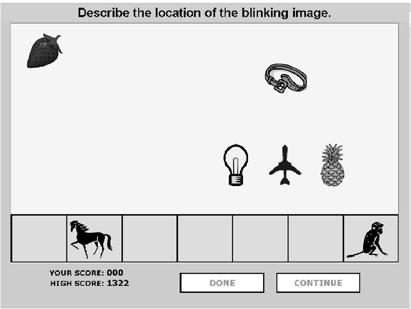
\includegraphics[scale=0.5]{images/columbia_games.jpg}
\caption{Juego de objetos del Columbia Games}
\label{objects_game}
\end{figure}


Cada sesión consistió de 14 tareas como ésta, cambiando los objetos y sus ubicaciones. En las primeras cuatro tareas, uno de los sujetos tomó el papel del Descriptor; en los siguientes cuatro invirtieron roles, y en las finales seis fueron alternando los roles de Descriptor y Seguidor.

\subsection{Anotaciones sobre comportamiento social}

Varios aspectos del comportamiento de los jugadores durante los juegos de objetos fueron anotados mediante la herramienta de crowdsourcing \emph{Amazon Mechanical Turk}. Cada anotador escuchó el audio correspondiente a una tarea del juego y tuvo que responder a varias preguntas sobre cada uno de los sujetos, entre las que se encuentran:

\begin{itemize}
  \item ¿el sujeto parece comprometido con el juego?
  \item ¿el sujeto dirige la conversación?
  \item ¿el sujeto contribuye para el éxito del equipo?
  \item ¿el sujeto alienta a su compañero?
  \item ¿el sujeto se expresa correctamente?
  \item ¿al sujeto no le agrada su compañero?
  \item ¿el sujeto le hace difícil hablar a su compañero?
  \item ¿el sujeto intenta acaparar la conversación?
\end{itemize}

\noindent Cada uno de estos audios fue puntuado por cinco anotadores, que respondieron por sí o por no para cada una de las preguntas. El puntaje que recibe cada una de las preguntas (a las cuales llamaremos a partir de ahora \emph{variables sociales}) consiste en la cantidad de respuestas afirmativas que recibió, teniendo un rango de 0 a 5. Por ejemplo, una tarea dada podría tener puntaje 3 para la variable social `el sujeto A se expresa correctamente' o puntaje 5 para la variable `el sujeto B dirige la conversación'.

\subsection{Extracción de variables acústico/prosódicas}

La herramienta \emph{Praat} fue utilizada para extraer automáticamente las variables \ap del corpus. Las variables que medimos fueron el tono, la intensidad, la proporción de vocalizaciones, jitter, shimmer, cantidad de sílabas, cantidad de fonemas, y la proporción de ruido sobre armónicos. Estos atributos fueron medidos en cada uno de los segmentos de habla del corpus.

Repasemos algunos conceptos que necesitamos para definir las variables acústicas.

\begin{itemize}
  \item \emph{f0} refiere a la frecuencia fundamental de una onda, que es el recíproco del período de ésta. El \emph{tono} o \emph{pitch} es la percepción que tenemos de la frecuencia fundamental, que nos marca cuán agudos o graves son los sonidos.
  \item \emph{Intensity} refiere al volumen o intensidad de la onda. Ésta mide la amplitud de la onda, y es la percepción de cuán fuerte es el sonido.
  \item \emph{jitter y shimmer} se refieren, en un intervalo de tiempo, a los desplazamientos de la onda de la verdadera periodicidad y de la amplitud, respectivamente. Están asociadas con la percepción de la calidad de la voz.
  \item Un \emph{fonema} es la articulación simple de sonidos del habla, tanto de vocales como de consonantes. Ejemplos de fonemas son los sonidos de las letras u, a, s, k en español.
  \item El \emph{noise-to-harmonics ratio} (abreviado NHR) puede considerarse como una medida de calidad de la voz, que cuantifica la proporción de ruido que hay en ésta.
\end{itemize}


En la siguiente tabla resumimos estas features. Recordemos nuevamente que estas features son medidas en un intervalo de tiempo.

\begin{figure}[h!]
\centering

\begin{tabular} {|c|c|}
  \hline
  Variable & Descripción \\
  \hline
  \hline
  \FOMEAN & Valor medio de la frecuencia fundamental \\\hline
  \FOMAX  & Valor máximo de la frecuencia fundamental \\\hline
  \ENGMEAN & Valor medio de la intensidad \\\hline
  \ENGMAX & Valor máximo de la intensidad \\\hline
  \NOISETOHARMONICS & Noise-to-harmonics descripto anteriormente \\\hline
  \LOCALSHIMMER & Shimmer medido \\\hline
  \SYLAVG & Cantidad de sílabas por segundo \\\hline
  \PHONAVG & Cantidad de fonemas por segundo \\\hline
\end{tabular}
\end{figure}
